\documentclass[12pt]{article}
\usepackage[a4paper,left=27mm,right=27mm,top=24mm,bottom=22mm]{geometry}
\usepackage[space]{ctex}
\usepackage{graphicx}
\usepackage{float}
\usepackage{subfigure}
\usepackage{amsmath}
\usepackage{amsfonts,amssymb}
\title{\LARGE\textbf{ImagePyramid}}
\author{SA21010060 周俊亦}
\date{}

\begin{document}
	\maketitle
	\renewcommand{\abstractname}{Abstract}
	\begin{abstract}
		图像金字塔是图像多尺度调整表达的一种重要的方式,在计算机视觉和图像压缩中得到重要的应用。本报告调研并实现了一些图像的上采样和下采样方法,并将采样结果与原图像进行相似度测量。具体方法包括:基于最大值池化和高斯金字塔的下采样方法,基于拉普拉斯金字塔、最近邻插值和双线性插值的上采样方法,以及基于 PNSR 和 SSIM 的图像相似度测量。
	\end{abstract}
	
	\section{概述}
	图像金字塔是图像多尺度调整表达的一种重要的方式。图像金字塔方法的原理是:将图像分解为多尺度的金字塔图像序列: 低分辨率的图像在上层,高分辨率的图像在下层,以获得图像的多尺度特征。图像金字塔的应用对图像的特征提取以及图像压缩作出了重大贡献。\\
	
	
	有两种类型的金字塔经常出现在文献和应用当中:\\
	
	
	\textbf{高斯金字塔(Gaussian pyramid)}: 用来向下采样(主要)\\
	
	
	\textbf{拉普拉斯金字塔(Laplacian pyramid)}: 存储图像残差,用来从低分辨率图像重建未采样的高分辨率图像,可以对图像进行有效的还原,通常与高斯金字塔配对使用。
	
	\begin{figure}[H]
		\centering
		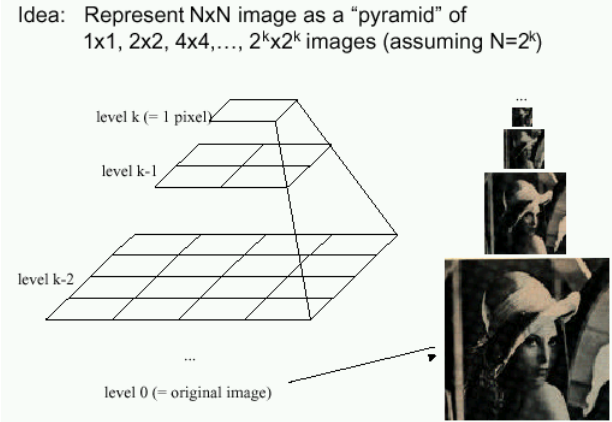
\includegraphics[width=3in]{./gausspyr.png}
		\centering
		\caption{Gaussian Pyramids}
	\end{figure}
	
	\begin{figure}[H]
		\centering
		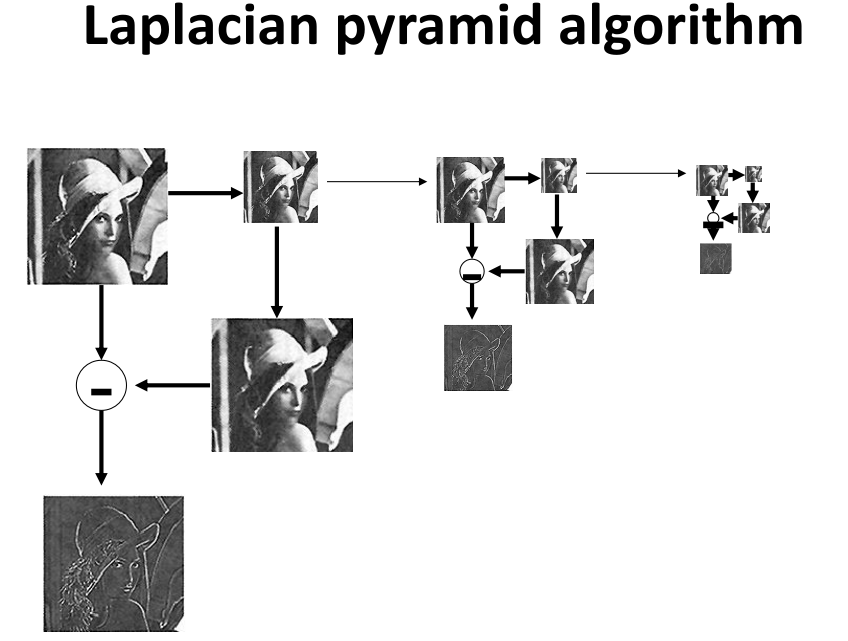
\includegraphics[width=3in]{./laplacepyr.png}
		\centering
		\caption{Laplacian pyramid}
	\end{figure}
	
	图像金字塔的精髓在于上采样和下采样算法,下文将介绍包括高斯金字塔和拉普拉斯金字塔在内的图像上采样和下采样方法。
	
	\section{下采样(Downsampling)}
		
		\subsection{高斯下采样}
		
		高斯金字塔下采样算法步骤为:\\
		
		
		1.利用低通滤波器对源图像进行平滑:高斯卷积核
		
		$$
		\frac{1}{16}\left[\begin{array}{ccccc}
			1 & 4 & 6 & 4 & 1 \\
			4 & 16 & 24 & 16 & 4 \\
			6 & 24 & 36 & 24 & 6 \\
			4 & 16 & 24 & 16 & 4 \\
			1 & 4 & 6 & 4 & 1
		\end{array}\right]
		$$
		
		2.对平滑后的图像进行下采样:删除偶数列和偶数行
		
		\subsection{最大值池化(Max-pooling)}
		最大池化(max-pooling)即取局部接受域中值最大的点。以 $2\times2$ 邻域为例,最大池化将保留$2\times2$ 邻域中值最大的像素点。
		
		\begin{figure}[H]
			\centering
			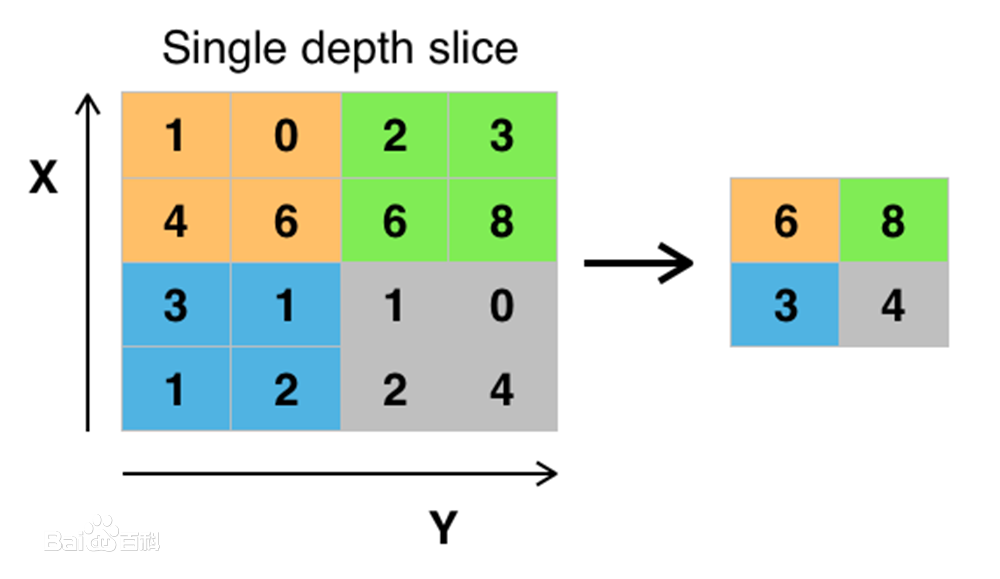
\includegraphics[width=3.5in]{./maxpool.png}
			\centering
			\caption{Max-Pooling}
		\end{figure}
		
		相比于高斯下采样和均值池化,最大池化能更多的保留图片的纹理信息。
		
	\section{上采样(Upsampling)}
	
	\subsection{拉普拉斯金字塔}
	拉普拉斯上采样是高斯下采样的逆过程。具体步骤为:\\
	
	1.在偶数行和和偶数列以0填充
	
	2.用下采样时用 $4$ 倍的高斯核卷积图像
	
	\subsection{最近邻插值}
	最近邻插值在图像放大时补充的像素取最临近的像素的值。由于方法简单,计算速度非常快。
	
	设原始图像为$I$,放大后图像为$I^{\prime}$,假设放大率为 $\alpha$ ,则最近邻插值公式为:
	
	$$
	I^{\prime}(x, y)=I\left(\left[\frac{x}{\alpha}\right],\left[\frac{y}{a}\right]\right)
	$$
	
	\begin{figure}[H]
		\centering
		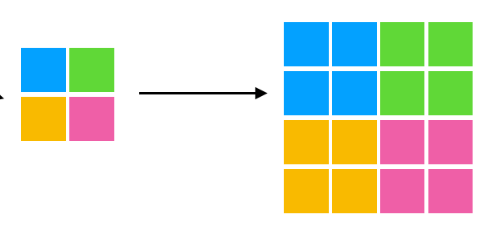
\includegraphics[width=3.8in]{./nn.png}
		\centering
		\caption{NN}
	\end{figure}

	\subsection{双线性插值}
	
	设函数 $f(x, y)$ 满足 $x_{1} \leq x \leq x_{2}$ 且 $y_{1} \leq y \leq y_{2}$ 。\\ 
	
	
	对 $f\left(x, y_{1}\right)$ 和 $f\left(x, y_{2}\right)$ 使用线性插值:
	$$
	\begin{aligned}
		f\left(x, y_{1}\right) & \approx \frac{x_{2}-x}{x_{2}-x_{1}} f\left(x_{1}, y_{1}\right)+\frac{x-x_{1}}{x_{2}-x_{1}} f\left(x_{2}, y_{1}\right) \\
		f\left(x, y_{2}\right) & \approx \frac{x_{2}-x}{x_{2}-x_{1}} f\left(x_{1}, y_{2}\right)+\frac{x-x_{1}}{x_{2}-x_{1}} f\left(x_{2}, y_{2}\right)
	\end{aligned}
	$$
	
	对 $f(x, y)$ 使用双线性插值:
	$$
	\begin{aligned}
		f(x, y) & \approx \frac{y_{2}-y}{y_{2}-y_{1}} f\left(x, y_{1}\right)+\frac{y-y_{1}}{y_{2}-y_{1}} f\left(x, y_{2}\right) \\
		& \approx \frac{x_{2}-x}{x_{2}-x_{1}} \frac{y_{2}-y}{y_{2}-y_{1}} f\left(x_{1}, y_{1}\right)+\frac{x-x_{1}}{x_{2}-x_{1}} \frac{y_{2}-y}{y_{2}-y_{1}} f\left(x_{2}, y_{1}\right) \\
		&+\frac{x_{2}-x}{x_{2}-x_{1}} \frac{y-y_{1}}{y_{2}-y_{1}} f\left(x_{1}, y_{2}\right)+\frac{x-x_{1}}{x_{2}-x_{1}} \frac{y-y_{1}}{y_{2}-y_{1}} f\left(x_{2}, y_{2}\right)
	\end{aligned}
	$$
	
	\begin{figure}[H]
		\centering
		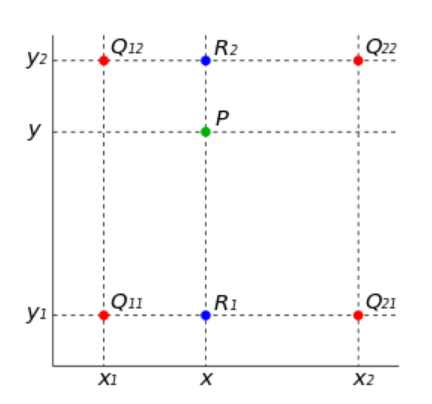
\includegraphics[width=3.8in]{./bilinear.png}
		\centering
		\caption{Bi-Linear}
	\end{figure}

	\section{图像相似度测量}
	
	\subsection{PSNR(Peak Signal to Noise Ratio)}
	峰值信噪比(PSNR)是衡量图像失真或是噪声水平的客观标准。2个图像之间PSNR值越大,则越相似。PSNR 定义为:
	
	$$
	P S N R=10 \log _{10}\left(\frac{M A X^{2}}{M S E}\right)
	$$
	
	其中,其中 $MAX^2$ 为图片可能的最大像素值。如果每个像素都由 8 位二进制来表示,那么就为 255。 $MSE$ 为均方差值:
	
	$$
	M S E=\frac{1}{m n} \sum_{i=0}^{n-1} \sum_{j=0}^{m-1}\|K(i, j)-I(i, j)\|^{2}
	$$
	
	\subsection{SSIM(Structural Similarity)}
	设 $x,y$ 为两个图像,SSIM 描述两个图像的相似性.
	
	$$
	\operatorname{SSIM}(x, y)=\frac{\left(2 \mu_{x} \mu_{y}+c_{1}\right)\left(2 \sigma_{x y}+c_{2}\right)}{\left(\mu_{x}^{2}+\mu_{y}^{2}+c_{1}\right)\left(\sigma_{x}^{2}+\sigma_{y}^{2}+c_{2}\right)}
	$$
	
	其中,
	$u_{x}$ 为 $x$ 的均值,
	$u_{y}$ 为 $y$ 的均值,
	$\sigma_{x}^{2}$ 为 $x$ 的方差,
	$\sigma_{y}^{2}$ 为 $y$ 的方差,
	$\sigma_{x y}$ 为 $x$ 和 $y$ 的协方差,
	$c_{1}=\left(k_{1} L\right)^{2}, c_{2}=\left(k_{2} L\right)^{2}$ 为两个常数, 避免除零,
	$L$ 为像素值的范围, $(0,255)$。
	$k_{1}=0.01, k_{2}=0.03$ 为默认值
	
	
	\section{实验分析}
	实验使用 Qt5.12.2 与 OpenCV3.4.15 进行算法验证,使用 gcc 编译生成。
	
		\subsection{程序界面}
	\begin{figure}[H]
		\centering
		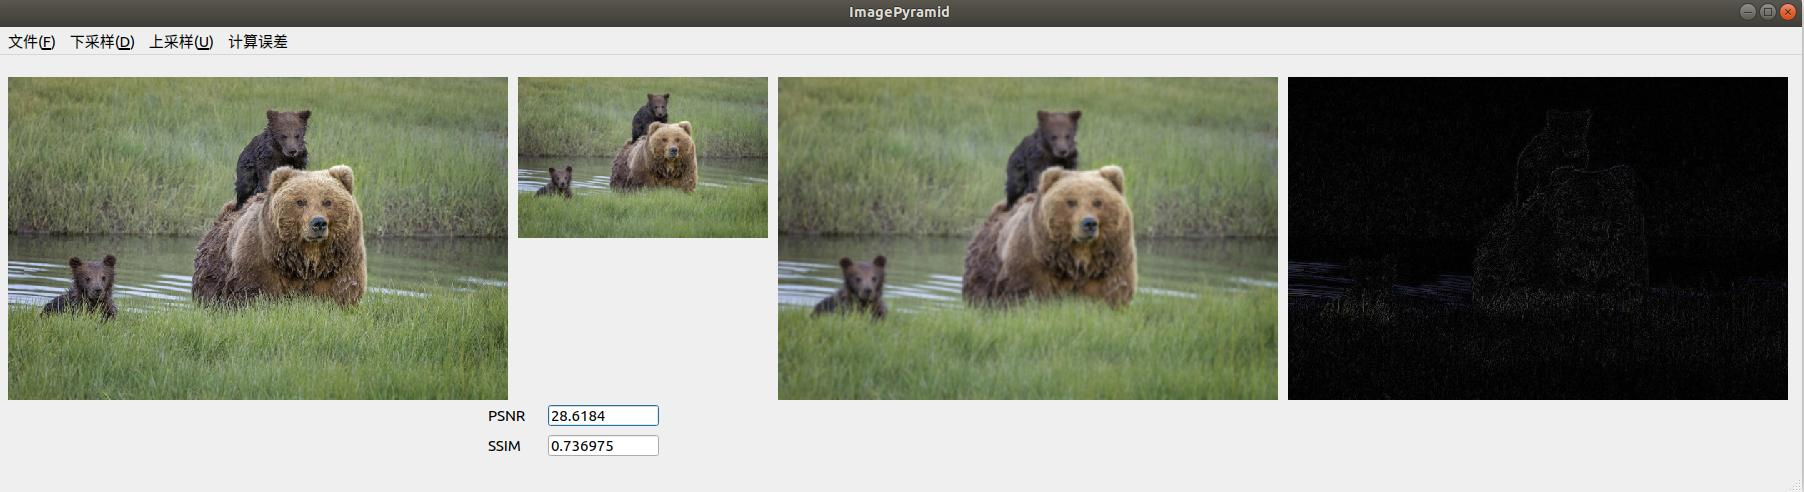
\includegraphics[width=6in]{./ui.png}
		\centering
		\caption{程序界面}
	\end{figure}
	
	用户可以选择下采样与上采样方法,选择计算误差可以生成差值图像,并计算“下采样+上采样”组合迭代一次后结果图像与原图像的 PNSR 与 SSIM 值。
	
	\subsection{Examples}
	
	\subsubsection{下采样方法对比}
	
	\begin{figure}[H]
		\centering
		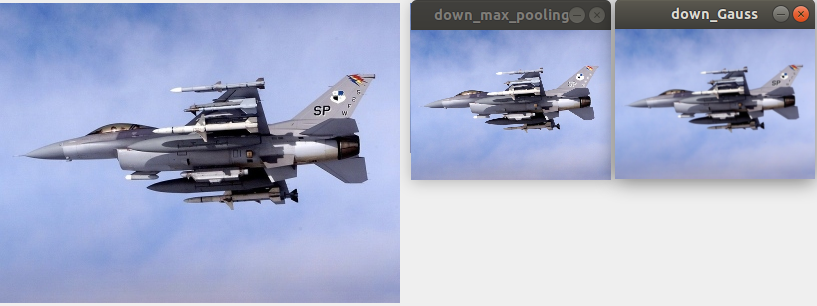
\includegraphics[width=6in]{./1.png}
		\centering
		\caption{Guassion vs Max-pooling}
	\end{figure}
	图例展示了同一图片在最大池化与高斯降采样算法下的对比,明显发现,最大值池化的纹理更加尖锐,印证了先前介绍时的观点,相比于高斯下采样和均值池化,最大池化能更多的保留图片的纹理信息。
	
	\subsubsection{上采样方法对比}
	
	\begin{figure}[H]
		\centering
		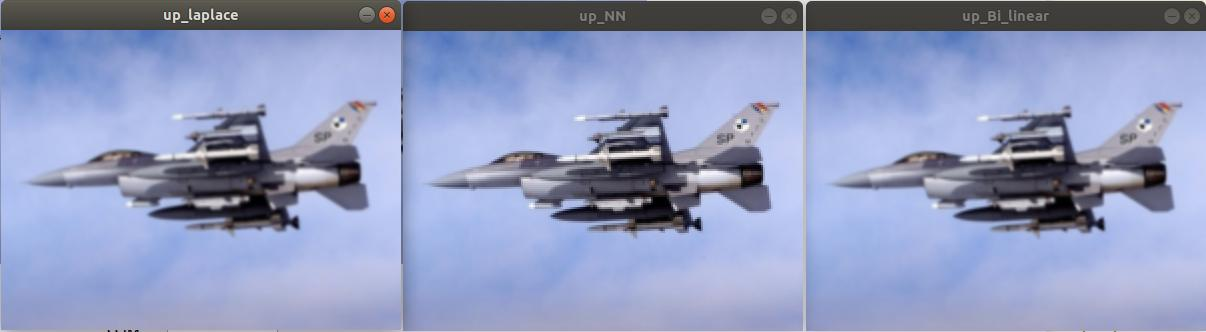
\includegraphics[width=6in]{./2.png}
		\centering
		\caption{Upsampling method comparison}
	\end{figure}

	图例展示了同一图片在高斯降采样算法后,进行三种不同上采样算法的对比。中间的图片为最近邻插值算法的上采样结果,可以明显发现,最近邻插值有肉眼可见的锯齿,而利用高斯卷积核的拉普拉斯上采样和双线性插值更加平滑。
	
	\subsubsection{相似度测量}
	实验将两幅图像用作示例,测试了上采样与下采样的不同组合,得出表格数据如下。
	
	\begin{figure}[H]
		\centering
		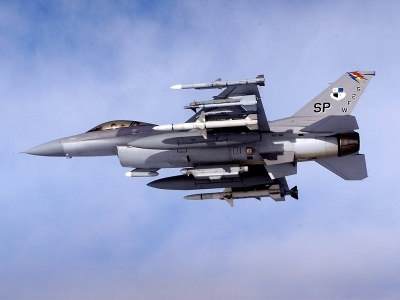
\includegraphics[width=3in]{./airplane.jpg}
		\centering
		\caption{原图像}
	\end{figure}
	
	\begin{table}[H]
		\centering
		\begin{tabular}{|c|c|c|c|c|}
			\hline
			& Laplace  & NN       & Bi-Linear \\ \hline
			PSNR & 24.9717  & 24.9692  & 25.8196   \\ \hline
			SSIR & 0.905043 & 0.913758 & \textbf{0.92046}   \\ \hline
		\end{tabular}
	\caption{Max-Pooling}
	\label{}
	\end{table}
	
	\begin{table}[H]
		\centering
		\begin{tabular}{|c|c|c|c|c|}
			\hline
			& Laplace  & NN      & Bi-Linear \\ \hline
			PSNR & \textbf{27.5714}  & 26.7464 & 26.9712   \\ \hline
			SSIR & 0.917735 & 0.91261 & 0.912679  \\ \hline
		\end{tabular}
	\caption{Guassion Pyramid}
	\label{}
	\end{table}
	
	\begin{figure}[H]
		\centering
		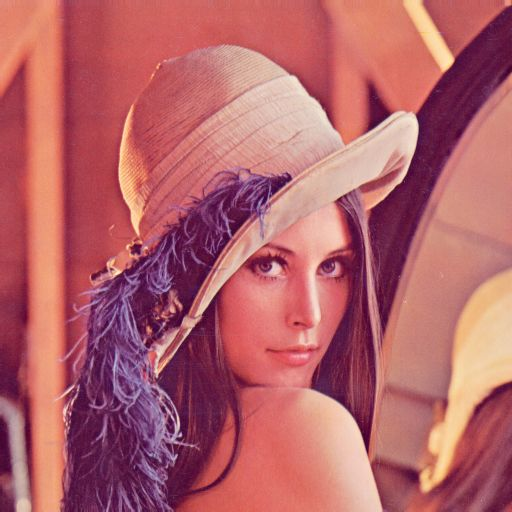
\includegraphics[width=3in]{./Lena.jpg}
		\centering
		\caption{原图像}
	\end{figure}
		
	\begin{table}[H]
		\centering
		\begin{tabular}{|c|c|c|c|c|}
			\hline
			& Laplace  & NN       & Bi-Linear   \\ \hline
			PSNR & 27.7809  & 27.8411  & 28.8432     \\ \hline
			SSIR & 0.880357 & 0.900359 & \textbf{0.913502}    \\ \hline
		\end{tabular}
	\caption{Max-Pooling}
	\label{}
	\end{table}
	
	\begin{table}[H]
		\centering
		\begin{tabular}{|c|c|c|c|c|}
			\hline
			& Laplace  & NN       & Bi-Linear   \\ \hline
			PSNR & \textbf{30.6814}  & 29.396   & 29.7136     \\ \hline
			SSIR & 0.883083 & 0.872125 & 0.873158    \\ \hline
		\end{tabular}
	\caption{Guassion Pyramid}
	\label{}
	\end{table}
	
	可以发现,在相同下采样的图像上,拉普拉斯金字塔与双线性插值算法的结果总体来说比最近邻插值要好。在下采样算法的选择上,高斯金字塔算法总体来说比最大值池化要好,最大值池化丢失了更多信息。
	
	从 PSNR 指标来说,在所有示例中,高斯金字塔与拉普拉斯金字塔配合使用,结果图像与原图像相似度最高。
	
	从 SSIM 指标来说,在所有示例中,最大值池化与双线性插值配合使用,结果图像与原图像相似度最高。
	
	以下将对上述结果作出可能的猜测。
	
	从理论角度来说, \textbf{PNSR 考虑峰值信噪比,考虑均方差值};而 \textbf{SSIM 考虑图像的亮度,对比度和结构},这些信息有很大部分存在于图像的纹理中。
	
	因此,\textbf{PSNR 反映了图像的"协调性"},这可能是为什么在 PSNR 指标看来,使用\textbf{倾向均值}的高斯金字塔下采样算法,能使结果图像与原图像相似度最高。
	
	而\textbf{SSIM 反映了图像的组成结构},这可能是为什么在 SSIM 指标看来,使用\textbf{倾向提取尖锐边缘}的最大值池化下采样算法,能使结果图像与原图像相似度最高。
	
	
	\section{实验总结}
	本次实验对图像缩放进行了多种算法实验,对图像结构的理解更多了。通过图像相似度评价标准的调研,也了解到了很多关于图像评价标准的知识。
	
	附睿客网代码链接:
	
	链接:https://rec.ustc.edu.cn/share/2e82dee0-448a-11ec-a7dc-8389fea65c67
	
	\begin{thebibliography}{99}
	
		[1]各类网页
		
	\end{thebibliography}
\end{document}

